\begin{figure*}[!htb]
	\centering
	%\hline
	\begin{subfigure}[t]{0.4\textwidth}
		\centering
		\caption{}
		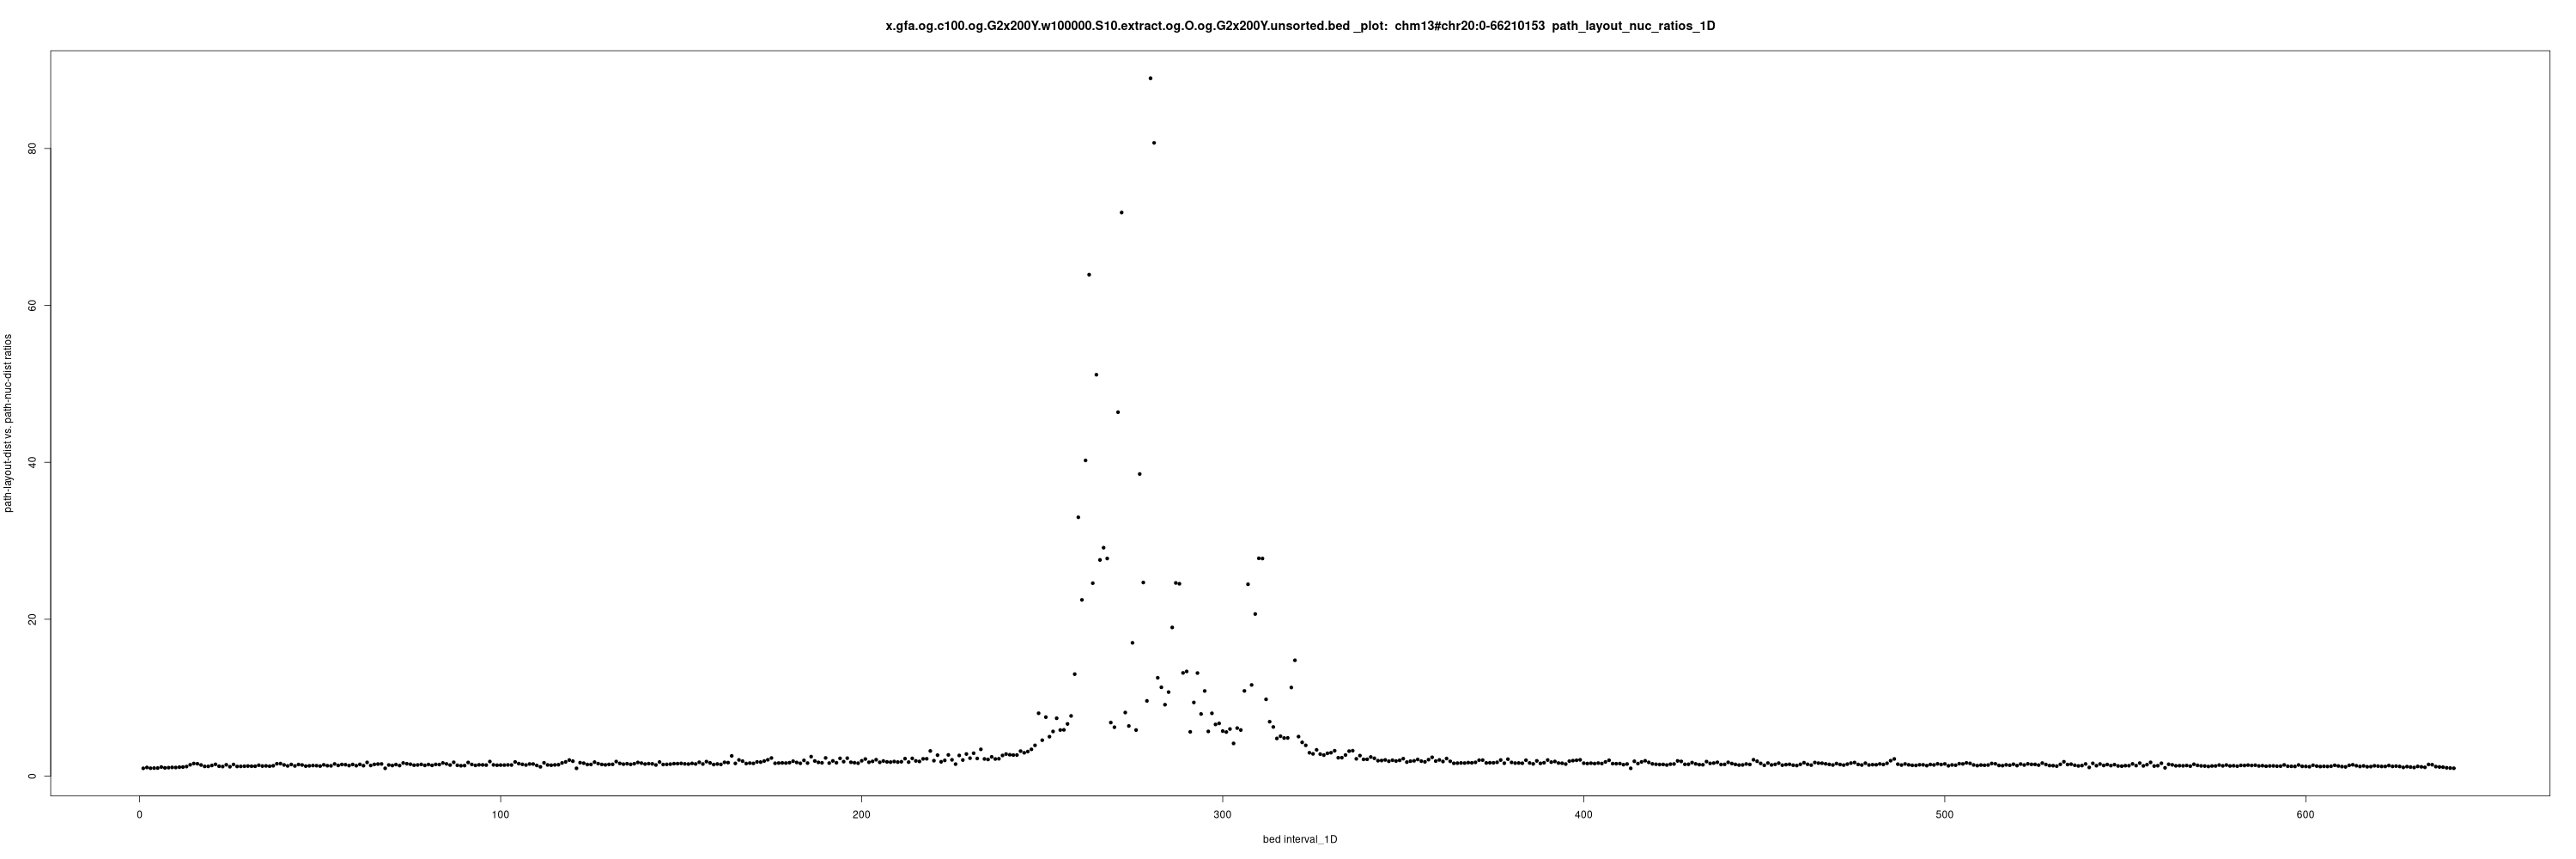
\includegraphics[width=\linewidth]{fig/tension/tension_bed.png}
		\label{fig:tension_bed}
	\end{subfigure}
	\begin{subfigure}[t]{0.4\textwidth}
		\centering
		\caption{}
		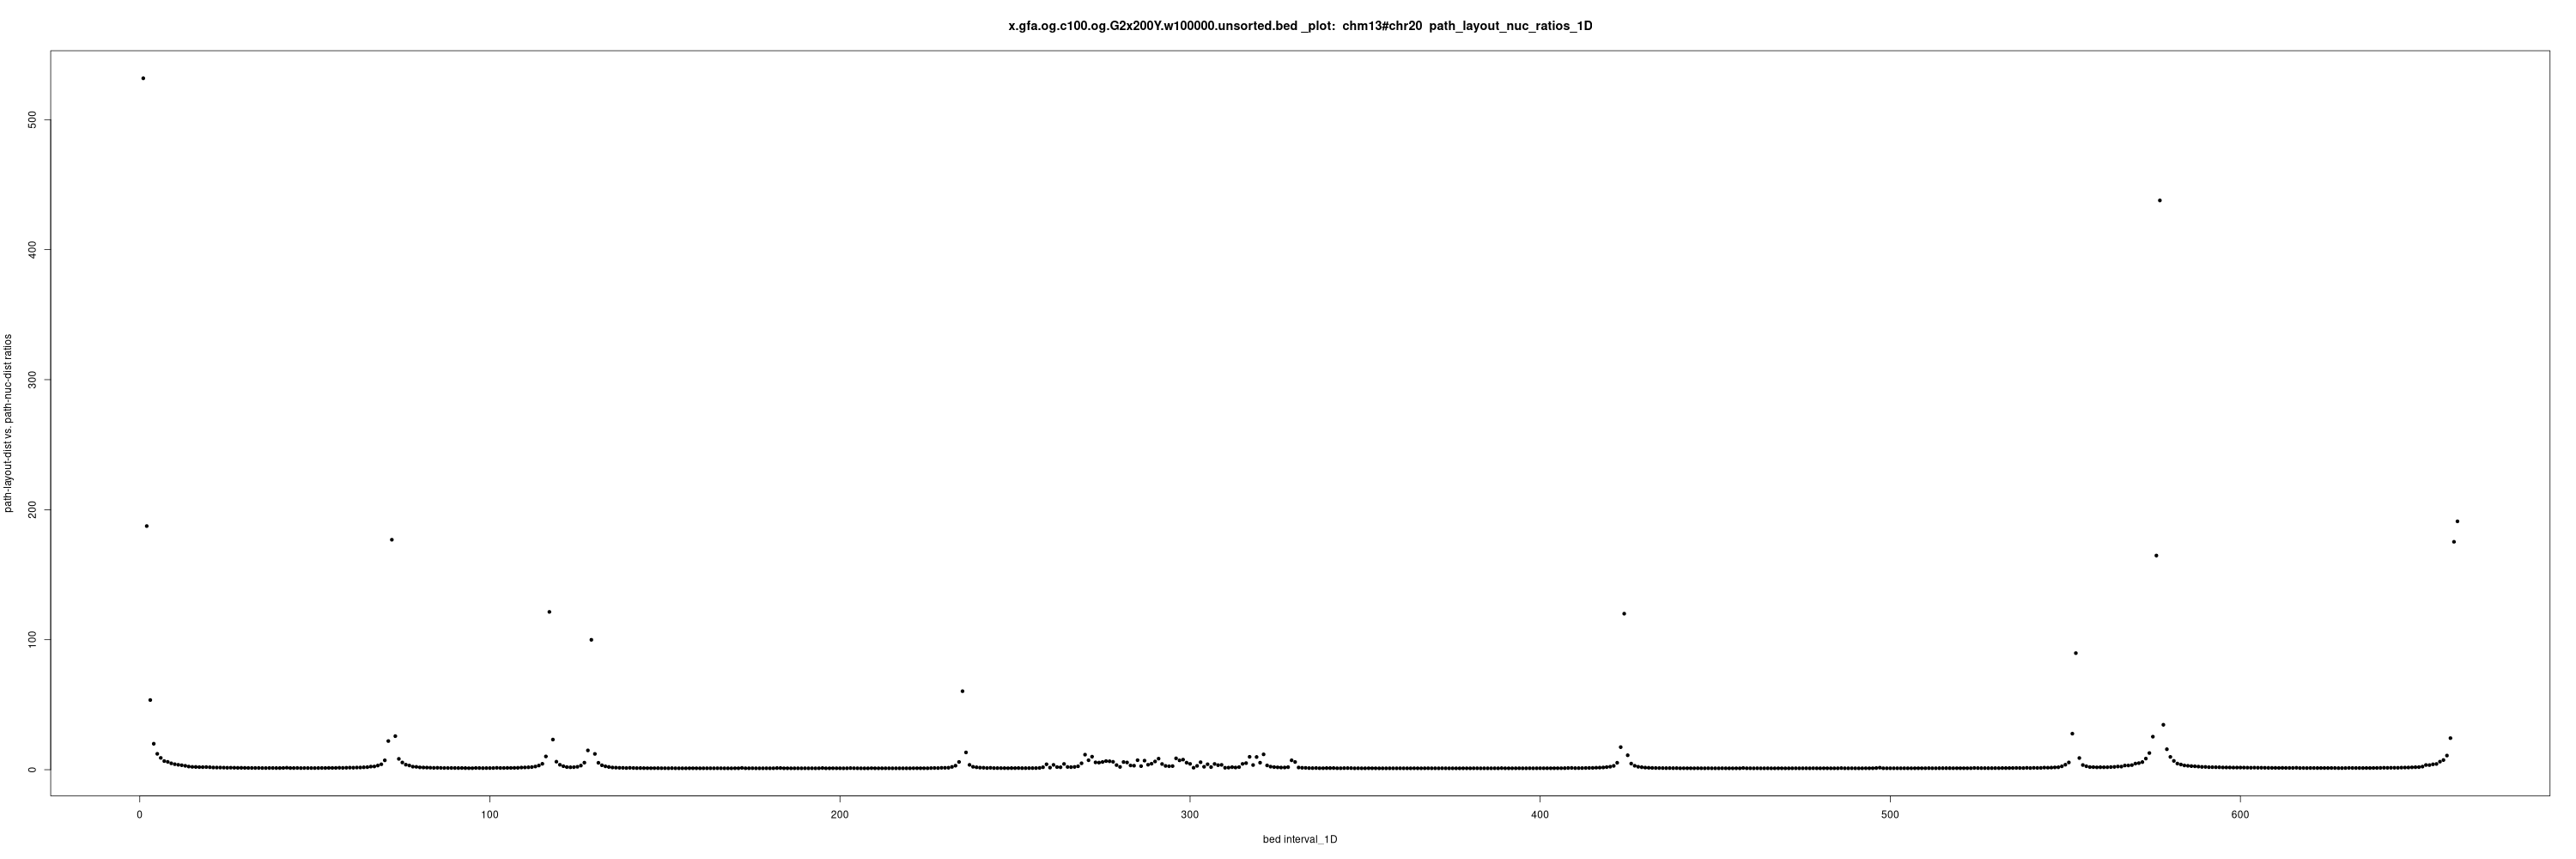
\includegraphics[width=\linewidth]{fig/tension/tension_bed_relaxed.png}
		\label{fig:tension_extracted}
	\end{subfigure}
\\
	%\smallskip
	\begin{subfigure}[t]{0.1\textwidth}
		\centering
		\caption{}
		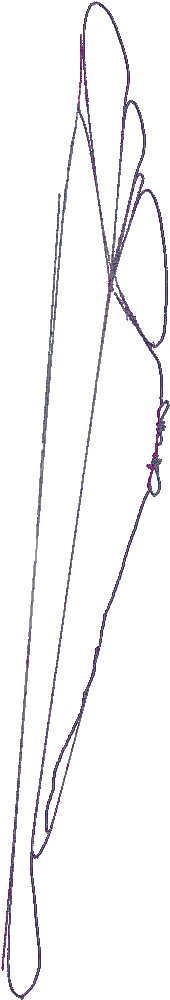
\includegraphics[width=\linewidth]{fig/tension/layout.png}
		\label{fig:tension_draw}
	\end{subfigure}
	\begin{subfigure}[t]{0.1\textwidth}
		\centering
		\caption{}
		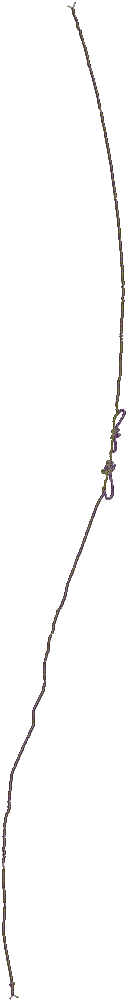
\includegraphics[width=\linewidth]{fig/tension/layout_relaxed.png}
		\label{fig:tension_draw_extracted}
	\end{subfigure}
	\caption{
		Detecting tension and relaxing a pangenome graph.
		\textbf{(a)} Tension detection before relaxation. \textbf{(b)} Tension detection after relaxation. \textbf{(c)} Folded 2D before relaxation. \textbf{(d)} Linearized 2D after relaxation.
	}
	\label{fig:tension}
\end{figure*}